\subsubsection{Sensor de pH}
O sensor de pH da água é de extrema importância para o projeto  pois monitora um dos índices de qualidade da água especificados pela ANA(agência nacional de águas). 

Para aplicações industriais, o método de medição de pH mais empregado é o eletrodo de vidro. Os eletrodos de pH possuem basicamente o mesmo funcionamento que as baterias: transferem uma tensão mínima que poderá ser detectada por um medidor ou um regulador de pH. A diferença é que os eletrodos de pH não produzem tensão de forma contínua, a não ser quando são introduzidos num líquido. Os sensores foram pesquisados principalmente nos sites \footnotemark \footnotetext{https://www.sparkfun.com}, \footnotemark \footnotetext{https://www.pololu.com} e \footnotemark \footnotetext{http://www.vernier.com}, o sensor a ser utilizado no projeto pode ser visto na imagem abaixo. 
	\begin{figure}[!htbp]
	  \centering
	  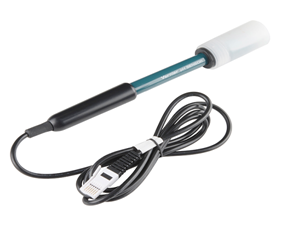
\includegraphics[scale=0.8]{editaveis/figuras/sensor_ph}
	  \caption[Sensor de pH]{Sensor de pH}
	  \label{sensor_ph}
	\end{figure}
	\FloatBarrier
Um ponto importante sobre os sensores de pH é o fato deles apresentarem erros de medição quando colocados em água destilada. Por este motivo, para se obter uma maior precisão na medição dos sensores, deve-se colocar o sensor de pH no tanque de água já adicionada de sais. Um dos fatores importantes para a escolha do Vernier sensor é o fato deste dispositivo ser compatível com softwares já existentes, além do fato dele possuir calibração via software, o que irá facilitar o manuseio do mesmo.

	A escolha do tipo de sensor de pH a ser utilizado depende também da temperatura do líquido a ser aferido. A faixa de temperatura do sensor escolhido é adequada para a aplicação, já que o sensor possui uma faixa de atuação de 5 a $80\,^{\circ}\mathrm{C}$. Como o sensor de pH funciona por meio de comparação, deve ser preparada uma solução para ser adicionada ao sensor. Recomenda-se a utilização de soluções de pH 4, 7 ou 10. A seguir, podem ser observadas as receitas das soluções de pH que podem ser utilizadas.

\begin{table}[h]
\centering 
\begin{tabular}{|c|p{12cm}|}\hline
pH 4,0 	& Adicionar 2.0 mL de 0.1 MHCl para cada 1000 mL de 0.1 M Hidrogenoftalato de potássio.\\\hline
pH 7,0 	& Adicionar 582 mL de 0.1 MNaOH para cada 1000 mL de 0.1 M di-hidrogenofosfato de potássio.\\\hline
pH 10,0 & 	Adicionar 214 mL de 0.1 MNaOH para 1000 mL de 0.05 M bicarbonato de sódio.\\ \hline
\end{tabular}

\caption{Preparo da solução para o sensor de pH}
\end{table}
\FloatBarrier

\begin{center}\textbf{Especificações técnicas do sensor de pH}
\end{center}

\begin{table}[h]
\centering 
\begin{tabular}{|c|p{9cm}|}\hline
Faixa de temperatura&5- $80\,^{\circ}\mathrm{C}$\\ \hline
Tensão de saída	&0.25 volts/pH\\ \hline
Faixa de atuação(pH)& pH 0-14\\ \hline
Preço&R\$ 78,95\\ \hline
Acurácia&+/- 0.2 unidades de pH\\ \hline
Tempo de resposta&	90\% da leitura acontece em 1 segundo\\ \hline
Resolução&13 bits\\ \hline
\end{tabular}

\caption{Especificações técnicas do sensor de pH}
\end{table}
\FloatBarrier